\BiChapter{环流的大偏差原理}{Large deviations of cycle currents}
大偏差关系到随机过程中小概率事件的长时涨落行为 \cite{varadhan1984large,den2000large}。本文在此考察了经验环流的大偏差。注意到周期边界条件下,单环马氏链的经验$LE$环流$(J_n^c)_{c \in \mathcal{C}}$定义在空间:
\begin{equation*}
    \mathcal{V} = \left\{(\nu^c)_{c\in \mathcal{C}}:\;\nu^c\geq 0,\;
    \sum_{c\in \mathcal{C}}|c|\nu^c  = 1\right\},
\end{equation*}
其中$|c|$表示环$c$的长度,即环$c$中状态数量。若满足下列三个条件\cite{varadhan1984large},则称经验$LE$环流$(J_n^c)_{c \in \mathcal{C}}$满足速率函数为$I_J:\mathcal{V}\rightarrow [0,\infty]$的大偏差原理:
\begin{itemize}
    \item 对$\forall \alpha \geqslant 0$,水平集$\{x \in \mathcal{V}: I_{J}(x) \leqslant \alpha\}$是紧的。
    \item 对任意开集$U \subset \mathcal{V}$,
        \begin{equation}\label{def1}
            \varliminf_{n\to\infty}\frac{1}{n}\log\mathbb{P}((J^c_n)_{c\in\mathcal{C}}\in U)\ge-\inf_{x\in U}I_J(x).
        \end{equation}
    \item 对任意闭集$F \subset \mathcal{V}$,
        \begin{equation}\label{def2}
            \varlimsup_{n\to \infty}\frac{1}{n}\log\mathbb{P}((J^c_n)_{c\in\mathcal{C}}\in F)\le -\inf_{x\in F}I_J(x).
        \end{equation}
\end{itemize}
从中可以看出,定义中的条件$(ii)$和$(iii)$表明对$\forall (\nu^c)_{c\in\mathcal{C}}\in\mathcal{V}$,满足:
\begin{equation}\label{LDP}
    \mathbb{P}(J^c_n=\nu^c,\;\forall c\in\mathcal{C})\propto e^{-n I_J(\nu)},\;\;\;n\to\infty,
\end{equation}
同样地,也可以定义经验$ST$环流的大偏差$(Q_c^{c_l})_{l \subset \mathcal{L}}$。

\BiSection{单环马氏链$LE$环流的大偏差}
首先讨论经验$LE$环流的大偏差原理。一般的马氏链中,速率函数的解析表达式$I_J$很难求出,因此下面将关注单环马氏链。单环系统中所有可能形成的环都已在 (\ref{cycle_space})中列出。

简化叙述推导过程,假设系统从状态$1$出发,这并不会降低命题的一般性。为了求出速率函数$I_J$,需要计算经验$LE$环流的联合分布。对任意环$c=(i_1, i_2, \cdots, i_s)$,令$\gamma^c = p_{i_1i_2}p_{i_2i_3}\cdots p_{i_si_1}$表示沿着环$c$产生的所有转移概率的乘积。对任意满足$\sum_{c \subset \mathcal{C}} |c| k^c=n$的负整数序列$k=(k^c)_{c\subset \mathcal{C}}$,因为假设周期边界条件,经验$LE$环流的联合分布为:

% 为了计算经验$LE$环流的速率函数,下面将证明(7)对某些离散值$\nu$成立。若环$c$形成的速度是$k^c$,那么环$c$的经验环流是$\nu^c = k^c /n$。为书写方便,记$k^i$替代$k^c$表示包含一个状态的环$c=(i)$的形成速度。类似的,记$k^{i,i+1}$表示环$c=(i,i+1)$形成的速度,记$k^+$表示环$c=(1, 2, \dots ,N)$形成的速度,$k^-$表示环$c=(1, N, \dots ,2)$形成的速度 (图1c)。类似地,本文用$\nu^i, \nu^{i,i+1}, \nu^+, \nu^-$表示相应的经验环流,用$J^i, J^{i, i+1}, J^{+}, J^{-}$表示相应的经验净环流。因为上述假设周期边界条件,对于某些$k=(k^c)_{c \in \mathcal{C}} \in \mathbb{N}^{2 \mathbb{N}+2}$,容易得到:
\begin{equation}\label{joint}
    \begin{split}
    \mathbb{P}\left(J^c_n=\nu^c,\;\forall c\in\mathcal{C}\right)
    =&\;\mathbb{P}\left(N^c_n=k^c,\;\forall c\in\mathcal{C}\right)\\
    =&\;|G_n(k)|\prod_{c\in\mathcal{C}}\left(\gamma^c\right)^{k^c},
    \end{split}
\end{equation}
其中$\nu^c = k^c/n$,$G_n(k)$表示$n$时刻可能形成的轨迹的集合,且称该类轨迹为容许轨迹。

为书写方便,若$c=(i)$是一状态环,则用$k^i$替代$k^c$;若$c=(i,i+1)$是两状态环,则用$k^{i,i+1}$表示;若$c=(1,2,\cdots,N)$是顺时针$N$状态环,则用$k^{+}$表示;若$c=(1,N,\cdots,2)$是逆时针$N$状态环,则用$k^{-}$表示。类似地,也用$\nu^i, \nu^{i,i+1}, \nu^+, \nu^-$表示相应的经验环流,用$J^i, J^{i, i+1}, J^{+}, J^{-}$表示相应的经验净环流。例如,对于三状态马氏链,如果序列$k=(k^c)_{c\subset \mathcal{C}}$为:
\begin{equation} \label{trajectory_ex}
    k^3 = k^{12} = k^{23} = k^- = 1, ~~~ k^1 = k^2 = k^{13} = k^+= 0
\end{equation}
那么再说时刻$n=8$,有8个容许轨迹,如表\ref{table:all possible trajectories}所示。

\begin{table}[htb!]
    \renewcommand\arraystretch{1.2}
    \begin{tabular}{cccccccccc}
    \hline
   $m$   & 0 & 1 & 2 & 3 & 4 & 5 & 6 & 7 & 8 \\\hline
   $\xi_m$& 1 & 3 & 3 & 2 & 3 & 2 & 1 & 2 & 1 \\\hline
   $\xi_m$& 1 & 3 & 2 & 3 & 3 & 2 & 1 & 2 & 1 \\\hline
   $\xi_m$& 1 & 3 & 3 & 2 & 1 & 2 & 3 & 2 & 1 \\\hline
   $\xi_m$& 1 & 3 & 2 & 1 & 2 & 3 & 3 & 2 & 1 \\\hline
   $\xi_m$& 1 & 2 & 3 & 3 & 2 & 1 & 3 & 2 & 1 \\\hline
   $\xi_m$& 1 & 2 & 3 & 2 & 1 & 3 & 3 & 2 & 1 \\\hline
   $\xi_m$& 1 & 2 & 1 & 3 & 3 & 2 & 3 & 2 & 1 \\\hline
   $\xi_m$& 1 & 2 & 1 & 3 & 2 & 3 & 3 & 2 & 1 \\\hline
    \end{tabular}\centering
    \caption{三状态马氏链中,8个容许轨迹,环$(3), (12), (23)$和$(1,3,2)$形成一次,环$(1), (2), (13)$和$(1,2,3)$没有形成过}
    \label{table:all possible trajectories}
\end{table}

接下来,计算容许轨迹的数量$G_n(k)$。基本的想法是在已部分排好序的轨迹中插入各种环。所有可能的插入方式的数量将会是容许轨迹的数量。计算过程分为三个步骤:

1)由于系统从状态$1$出发,第一步,选出初始状态是$1$的环,即$(1)$,$(1,2)$,$(1,N)$,$(1,2,\cdots,N)$,$(1,N,\cdots,2)$,并且插入到轨迹中。因为环$c$形成$k^c$次,所以步骤1)所有可能的插入方式的数量,即这些环的排列数为:
\begin{equation*}\label{formula:A1}
    A_1 = \binom{k^1+k^{12}+k^{1N}+k^{+}+k^{-}}{k^1,k^{12},k^{1N},k^{+},k^{-}}
    := \frac{(k^1+k^{12}+k^{1N}+k^{+}+k^{-})!}{k^1!\;k^{12}!\;k^{1N}!\;k^{+}!\;k^{-}!}.
\end{equation*}
对于 \ref{trajectory_ex}中的例子,步骤1)中所有可能的插入方式为图 \ref{figure:insertion}左部分所示。
\begin{figure}[htb!]
\centering
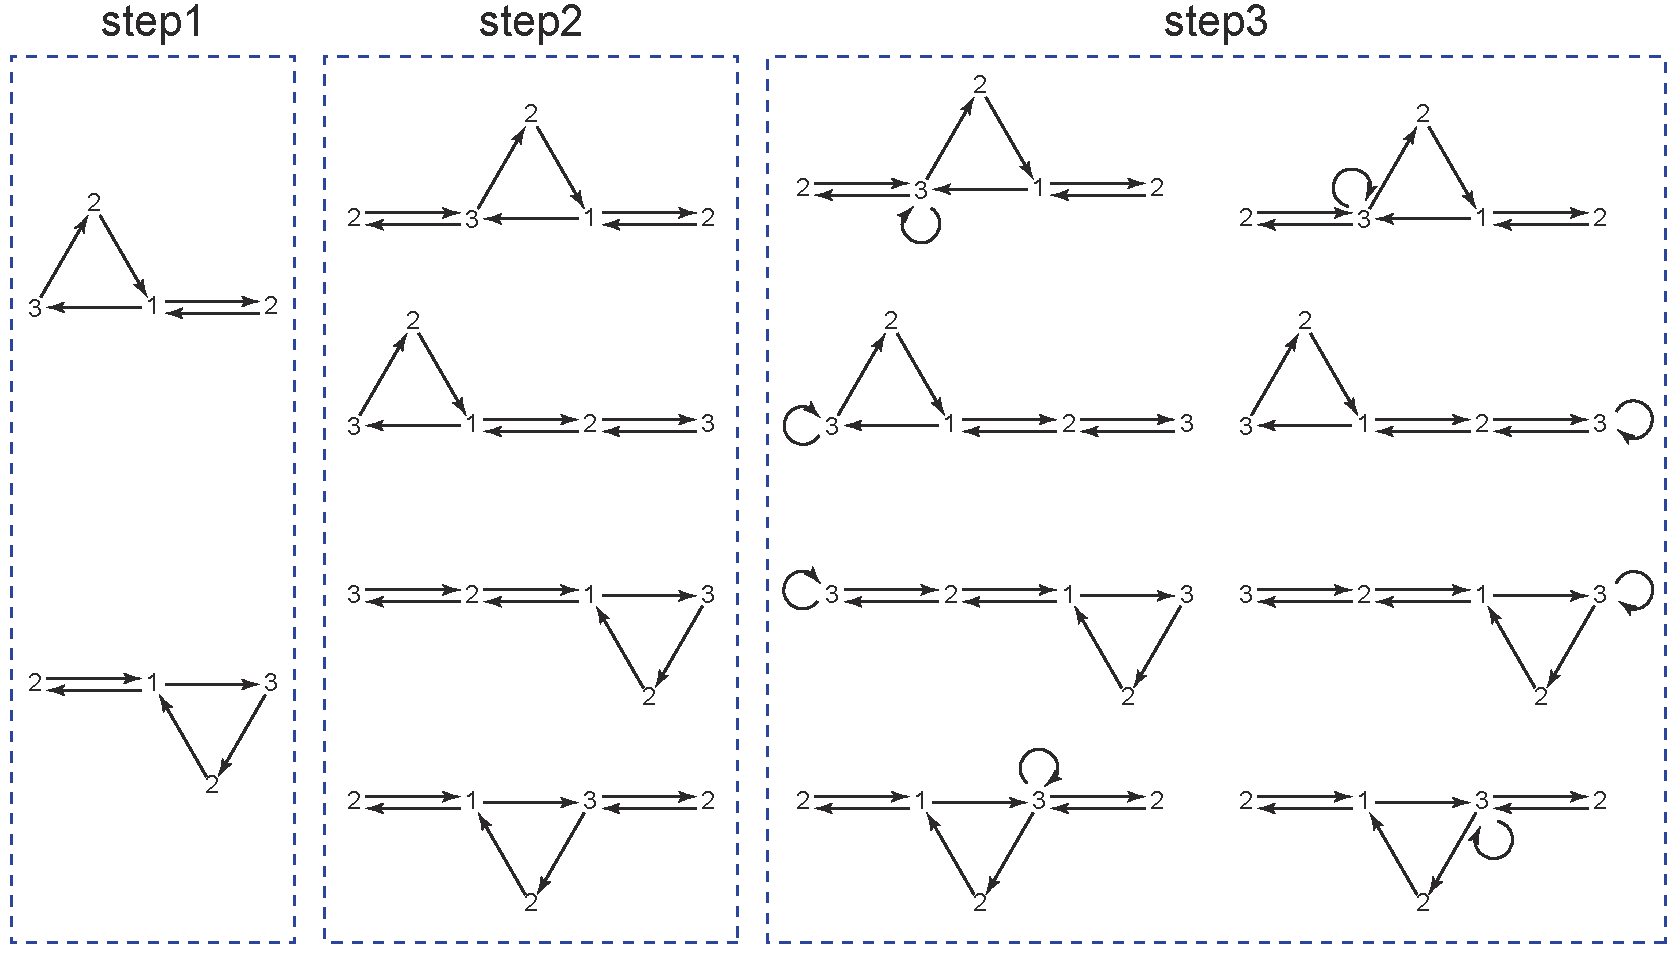
\includegraphics[scale=0.6]{chart/insertiongraph.pdf}
\caption{构建所有容允许轨迹的环插入法示意图。依然使用\ref{trajectory_ex}中的例子。环插入法分为三步:首先我们将所有包含初始状态的环插入轨迹,接下来我们将所有剩余的两状态循环插入轨迹,最后我们将所有剩余的单状态循环插入轨迹。经过这三步的环插入,找到了所有八个可允许的轨迹,这与表中所列的轨迹完全吻合。}
\label{figure:insertion}
\end{figure}

2)在轨迹中插入剩余的两状态环。仔细观察系统形成环$(i,i+1)$的情况,可能在状态$i$,也可能是$i+1$。例如,轨迹$\{1, 3, 2, 3, \cdots\}$,形成环$(2,3)$时,导出链是$[1, 3]$。对此,称这个环是在状态$3$处形成。相对比,轨迹$\{1,2,3,2, \cdots\}$,形成环$(2,3)$时,导出链是$[1, 2]$,因此称环是在状态$2$处形成的。

考虑两状态环$(i, i+1), 2\leqslant i \leqslant N-1$,令$l^i$和$m^i$分别表示在状态$i$和$i+1$处形成环$(i, i+1)$的数量,显然$l^i + m^i = k^{i, i+1}$。固定$l^i$和$m^i$,容许轨迹的数量可以计算得到。首先,在状态$2$处插入$l^2$个环$(2, 3)$,总共有$k^+ + k^{12}$个可能的位置可以插入,然而环$(1,2, \cdots, N)$和环$(1, 2)$已经在步骤1)中考虑。还要注意到,这些位置没有包含环$(1, N, \cdots, 2)$中的状态$2$,因此如果插入$(2,3)$,这个环将会在状态$3$处形成,而不是状态$2$。因此可能的插入方式数量是:
\begin{equation} \label{binom1}
    \binom{k^++k^{12}+l^{2}-1}{l^{2}}.
\end{equation}
接下来,把状态$3 \leqslant i \leqslant N$对应的$l^i$个环$(i, i+1)$插入轨迹中,且每个状态$i$总共有$k^+ + l^{i-1}$个可能的位置插入,这对应了环$(1, 2, \cdots, N)$和环$(i-1, i)$。因此可能的插入方式数量是:
\begin{equation} \label{binom2}
    \binom{k^++l^{i-1}+l^{i}-1}{l^{i}},\;\;\;3\le i\le N-1.
\end{equation}
目前,已经插入$l^i$个环$(i,i+1)$。结合 \ref{binom1}和 \ref{binom2},所有可能的插入方式的数量:
\begin{equation*}
    \prod_{i=2}^{N-1}\binom{l^{i}+l^{i-1}+k^{+}-1}{l^{i}}
\end{equation*}
其中$l^1:=k^{12}$。

同理,把状态$2 \leqslant i \leqslant N-1$对应的$m^i$个环$(i, i+1)$插入轨迹,所有可能的插入方式的数量:
\begin{equation*}
    \prod_{i=2}^{N-1}\binom{m^{i}+m^{i+1}+k^{-}-1}{m^{i}},
\end{equation*}
其中$m^N:=k^{N1}$。所有两状态的环就已经完全被插入。步骤 2)中所有可能的插入方式数量为:
\begin{equation*}
    A_2 = \sum_{l^{2}+m^{2}=k^{23}}\dots\sum_{l^{N-1}+m^{N-1}=k^{N-1,N}}
    \prod_{i=2}^{N-1}\binom{l^{i}+l^{i-1}+k^{+}-1}{l^{i}}\prod_{i=2}^{N-1}\binom{m^{i}+m^{i+1}+k^{-}-1}{m^{i}},
\end{equation*}
例子 \ref{trajectory_ex}中,步骤2)中的插入方式在图 \ref{figure:insertion}的中间部分。

3)最终把剩下的所有一状态的环插入轨迹中。对每个环$(i), 2 \leqslant i \leqslant N$,总共有$\sum_{c\ni i}k^c-k^i$个可选择的位置插入。因此步骤 3)总共的可能的插入方式数量为:
\begin{equation*}\label{formula:A3}
    A_3 = \prod_{i=2}^N\binom{\sum_{c\ni i}k^{c}-1}{k^{i}}.
\end{equation*}
例子 \ref{trajectory_ex}中,步骤3)中的插入方式在图 \ref{figure:insertion}的右部分。

结合上述三个步骤,最终可以得到容许轨迹的数量为:
\begin{equation}\label{trajectories}
    |G_n(k)|=A_1A_2A_3.
\end{equation}
为了得到更明确的速率函数表达式,先回顾$Stirling$公式:
\begin{equation*}
    \log n! = n\log n-n+O(\log n)=h(n)-n+O(\log n),
\end{equation*}
其中$h(x)=x \log x, x \geqslant 0$。记$k_i=\sum_{c\ni i}k^c$且$\nu_i=\sum_{c\ni i}\nu^c$,那么有:
\begin{equation}\label{log A1}
    \begin{split}
    \log A_1&=\log\frac{(k^1+k^{12}+k^{1N}+k^{+}+k^{-})!}{k^1!\;k^{12}!\;k^{1N}!\;k^{+}!\;k^{-}!}\\
    &= h(k_1)-h(k^1)-h(k^{12})-h(k^{1N})-h(k^+)-h(k^-)+O(\log n)\\
    &= n\left[h(\nu_1)-h(\nu^1)-h(\nu^{12})-h(\nu^{1N})-h(\nu^+)-h(\nu^-)\right]+O(\log n).
    \end{split}
\end{equation}
最后,估计$\log A_2$,令:
\begin{equation*}
    D = \{(l^i,m^i)_{2\le i\le N-1}:\;l^i,m^i\in\mathbb{N},\;l^i+m^i=k^{i,i+1}\}.
\end{equation*}
表示$l^i$和$m^i$可能的组合形成的集合。记$L = (l^i,m^i)\in D$, 令
\begin{equation*}
    B_L=\prod_{i=2}^{N-1}\binom{l^{i}+l^{i-1}+k^{+}-1}{l^{i}}\binom{m^{i}+m^{i+1}+k^{-}-1}{m^{i}}.
\end{equation*}
表示在给定$l^i$和$m^i$时,步骤 2)中插入方式的数量。易知$|D| \leqslant (n+1)^{N-2}$,因此,可以得到:
\begin{equation}\label{inequality}
    \max_{L\in D}B_L \le A_2 \le (n+1)^{N-2} \max_{L\in D}B_L,
\end{equation}
该式中还运用了$A_2 = \sum_{L\in D}B_L$。类似于 (11) 式,有:
\begin{equation}\label{log BL}
    \begin{split}
    \log B_L =&\;\sum_{i=2}^{N-1}[h(l^i+l^{i-1}+k^+)-h(l^i)-h(l^{i-1}+k^+)]\\
    &\;+\sum_{i=2}^{N-1}[h(m^i+m^{i+1}+k^-)-h(m^i)-h(m^{i+1}+k^-)]+O(\log n)\\
    =&\;\sum_{i=2}^{N-1}n[h(x^i+x^{i-1}+\nu^+)-h(x^i)-h(x^{i-1}+\nu^+)]\\
    &\;+\sum_{i=2}^{N-1}n[h(y^i+y^{i+1}+\nu^-)-h(y^i)-h(y^{i+1}+\nu^-)]+O(\log n),
    \end{split}
\end{equation}
其中$x^i = l^i/n$和$y^i = m^i/n$。对于给定的$\nu \in \mathcal{V}$,考虑其到处的空间:
\begin{equation*}
    V(\nu) = \left\{\left(x^{i},y^{i}\right)_{2\le i\le N-1}:\;x^i,y^i\geq0,\;x^{i}+y^{i}=\nu^{i,i+1}\right\},
\end{equation*}
且记$X = (x^i, y^i) \in V(\nu)$。定义函数:
\begin{equation}\label{formula:F}
    \begin{split}
    F_{\nu}(X)
    =&\sum_{i=2}^{N-1}\left[ h\left(x^{i-1}+\nu^+\right) + h\left(x^{i}\right) - h\left(x^{i-1}+x^{i}+\nu^+\right) \right] \\
    &+ \sum_{i=2}^{N-1} \left[h\left(y^{i}\right) + h\left(y^{i+1} +\nu^-\right)-h\left(y^{i} +y^{i+1} +\nu^-\right)\right].
    \end{split}
\end{equation}
那么联系(12)式的结果,可知:
\begin{equation}\label{log A2}
    \log A_2 = \max_{L\in D}\log B_L+O(\log n)
    = n\sup_{X\in V(\nu)}F_{\nu}(X)+O(\log n).
\end{equation}
结合\eqref{LDP}, \eqref{joint} 和 \eqref{trajectories}可得:
\begin{equation*}
    \begin{split}
    I_J(\nu) &= -\lim_{n\to\infty}\frac{1}{n}\log\mathbb{P}\left(J^c_n=\nu^c,\;\forall c\in\mathcal{C}\right)\\
    &= -\lim_{n\to\infty}\frac{1}{n}\left[\log A_1+\log A_2+\log A_3+\sum_{c\in\mathcal{C}}k^c\log\gamma^c\right].
    \end{split}
\end{equation*}
再联系\eqref{log A1}, \eqref{log A3},和 \eqref{log A2}式,可得:
\begin{equation}\label{ratefunction}
    \begin{split}
    I_J(\nu) =&\; \left[h\left(\nu^{12}\right)+h\left(\nu^{1N}\right)
    +h\left(\nu^+\right)+h\left(\nu^-\right)-h\left(\nu^{12}+\nu^{1N}+\nu^++\nu^-\right)\right] \\
    &\;+\inf_{X\in V(\nu)}F_{\nu}(X)+\sum_{i\in S}\left[ h\left(\nu_i-\nu^i\right)+h\left(\nu^i\right)
    -h\left(\nu_i\right)\right]-\sum_{c\in\mathcal{C}}\nu^c\log\gamma^c,
    \end{split}
\end{equation}
其中$h(x) = x \log x$且$\nu_i=\sum_{c\ni i}\nu^c$。这就是经验$LE$完整的环流速率函数表达式。该式中的$\inf_{X\in V(\nu)}F_{\nu}(X)$难以直接计算,不过可以通过拉格朗日乘子法得到。在附录 A 中,证明了
\begin{equation*}
    \inf_{X\in V(\nu)}F_{\nu}(X) = F_{\nu}(x^i,y^i),
\end{equation*}
其中$x^1=\nu^{12}$,$x^N=0$,$y^1=0$,并且$y^N=\nu^{1N}$。

上述论证,都是基于系统的初始状态是$1$,自然会联想到,基于其他初始分布,速率函数的表达式是否与其一致。附录 B 给出了速率函数不依赖初始状态的证明,由 \eqref{ratefunction} 的形式,可以看出这是一个极不平凡的结论。

为建立经验$LE$环流大偏差原理,依然要证明速率函数的水平集是紧的,也就是验证条件 \eqref{def1} 和 \eqref{def2}。大偏差原理严格的证明在附录 \ref{appendix:LDP} 中给出。总结上面的论述,可以得到下面的定理

\begin{theorem}\label{thm:LDP}
    单环马氏链的经验环流$(J^c_n)_{c\in\mathcal{C}}$满足大偏差原理,并且相应的速率函数$I_J:\mathcal{V}\to [0,\infty]$满足上式 \eqref{ratefunction}. 速率函数$I_J$满足有界性,连续性和凸性。并且,速率函数$I_J$并不依赖初始分布的选择。
\end{theorem}

一般单环马氏链的速率函数表达式 \eqref{ratefunction} 十分复杂。不过,如果令状态$1$到状态$N$的转移概率为 0,或者只考虑三状态的马氏链。若$N=3$,则速率函数可以化简为:(证明细节见 \ref{appendix:threestate})
\begin{align*}
    I_J(\nu) =
    \sum_{i\in S} \left[\nu^{i}\log \left(\frac{\nu^{i}/\nu_i}{J^i/J_i}\right) + (\nu_i - \nu^i)\log \left(\frac{(\nu_i - \nu^i)/\nu_i}{(J_i - J^i)/J_i} \right)
    \right]
    + \sum_{c\in\mathcal{C},|c|\neq 1} \nu^{c} \log \left(\frac{\nu^{c}/\tilde{\nu}}{J^c/\tilde{J}}\right) ,
\end{align*}
其中
\begin{align*}
    \tilde{\nu} &=\sum_{c\in\mathcal{C},|c|\neq 1}\nu^{c}
    = \nu^{12}+\nu^{13}+\nu^{23}+\nu^++\nu^-,\\
    \tilde{J} &=\sum_{c\in\mathcal{C},|c|\neq 1}J^{c}
    = J^{12}+J^{13}+J^{23}+J^++J^-.
\end{align*}
若$p_{1N}=0$,速率函数可以化简为(证明细节见 \ref{appendix:threestate}):
\begin{equation}\label{lack}
    \begin{split}
        I_J(\nu) = \sum_{i\in S}\Bigg[&\;\nu^i\log\left(\frac{\nu^i/\nu_i}{J^i/J_i}\right)
        +\nu^{i,i+1}\log\left(\frac{\nu^{i,i+1}/\nu_i}{J^{i,i+1}/J_i}\right)\\
        &\;+\left(\nu^{i-1,i}+\nu^+\right)\log\left(\frac{\left(\nu^{i-1,i}+\nu^+\right)/\nu_i}
        {\left(J^{i-1,i}+J^+\right)/J_i}\right)\Bigg].
    \end{split}
\end{equation}
最好,考虑经验经验净$LE$环流$(\tilde{J}^{c}_n)_{c\in\mathcal{C}}$的大偏差原理。因为$\tilde{J}^c_n = 0, |S|=1,2$且$\tilde{J}^+_n = -\ {J}^-_n$,所以只需要考虑环$(1, 2, \cdots ,N)$的经验净环流。那么由收缩原理可以得到:
\begin{equation}\label{tilde I J}
	\begin{split}
		\mathbb{P}\left(\tilde{J}^{+}_n = x\right)
		&=\;\mathbb{P}\left(J^{+}_n-J^{-}_n = x\right)\\
		&=\;\sum_{\nu^{+}-\nu^{-}=x}\mathbb{P}\left(J^{c}_n=\nu^{c},\forall c\in\mathcal{C}\right)\\
		&\propto\sum_{\nu^{+}-\nu^{-}=x} e^{-nI_J(\nu)}.
	\end{split}
\end{equation}
由此说明$\tilde{J}^+_n$满足大偏差原理, 相应的速率函数$I_{\tilde{J}}:\mathbb{R}\rightarrow[0,\infty]$为:
\begin{equation*}
	I_{\tilde{J}}(x)=\inf_{\{\nu\in\mathcal{V}:\nu^{+}-\nu^{-}= x\}}I_J(\nu).
\end{equation*} 
从上述表达式,也可以看出$I_{\tilde{J}}$与初始分布的选择无关。

\subsection{一般马氏链的$ST$环流的大偏差}

$ST$经验净环流的大偏差,以及速率函数的对称性已经在文献 \cite{bertini2015flows} 中有过相关介绍。本文将着重研究经验$ST$环流的大偏差原理,涉及对经验测度部分可参考 \cite{den2008large}。

$n$时刻的对经验测度$R_n:E\rightarrow[0,1]$,可以定义为
\begin{equation*}
R_n(i,j) = \frac{1}{n}\sum_{m=1}^n1_{\{\xi_{m-1}=i,\xi_m=j\}},
\end{equation*}
其中假设周期边界条件$X_0 = X_n$。显然$R_n(i,j)$表示边$\langle i,j\rangle$形成的速度。注意到,对经验测度$R_n$处于空间
\begin{equation*}
\mathcal{M} = \left\{R:E\rightarrow[0,1]:\;\sum_{i,j\in S}R(i,j) = 1,\;
\sum_{j\in S}R(i,j)=\sum_{j\in S}R(j,i)\right\}.
\end{equation*}
众所周知,对经验测度满足下面的大偏差原理:
\begin{equation*}
\mathbb{P}(R_n(i,j)=R(i,j),\;\forall\langle i,j\rangle\in E)\propto e^{-nI_{\mathrm{pair}}(R)},\;\;\;n\to\infty,
\end{equation*}
上式中的速率函数$I_{\mathrm{pair}}:\mathcal{M}\rightarrow[0,\infty]$的表达式为
\begin{equation*}
I_{\mathrm{pair}}(R) = \sum_{\langle i,j\rangle\in E}R(i,j)\log\frac{R(i,j)}{R(i)p_{ij}}
\end{equation*}
其中$R(i)=\sum_{j\in S}R(i,j)$,可以看到,对经验测度的速率函数可以表示为有着明显的相对熵形式。给定生成树$T$,定义在空间$E$上的函数$H^{c_l}$为:
\begin{equation*}\label{cycle function2}
H^{c_l}(i,j)
    =\left\{\begin{aligned}
    1, &   && \text{if } \langle i,j\rangle \in c_l \text{ and }\langle i,j\rangle \in T, \text{ or } \langle i,j\rangle=l,\\
    -1,&   && \text{if } \langle i,j\rangle\notin c_l,\langle j,i\rangle \in c_l,\text{ and }\langle i,j\rangle \in T,\\
    0, &   && \text{otherwise}.\\
    \end{aligned}\right.
\end{equation*}
对经验测度可以被分解为下面$ST$环流的加权和:
\begin{equation*}
R_n(i,j) = \sum_{c_l\in\mathcal{L}}H^{c_l}(i,j)Q^{c_l}_n,
\end{equation*}
且由文献 \cite{kalpazidou2007cycle}可知,该分解是唯一的。那么有:
\begin{equation*}
    \mathbb{P}(Q_n^{c_l}=\mu^{c_l},\;\forall c_l\in\mathcal{L})
    =\mathbb{P}\left(R_n(i,j)=\sum_{c_l\in\mathcal{L}}\mu^{c_l}H^{c_l}(i,j),\;\forall\langle i,j\rangle\in E\right)
    \propto e^{-n I_{\mathrm{pair}}\left(\sum_{c_l\in\mathcal{L}}\mu^{c_l}H^{c_l}\right)}.
\end{equation*}
这表明 ST 经验环流$(Q_n^{c_l})_{c_l\in\mathcal{L}}$满足大偏差原理,相应的速率函数$I_Q:\mathcal{M}\rightarrow[0,\infty]$为:
\begin{equation}\label{formula:I_Q}
I_Q(\mu)=I_{\mathrm{pair}}\left(\sum_{c_l\in\mathcal{L}}\mu^{c_l}H^{c_l}\right).
\end{equation}
最终,考虑 ST 经验净环流$(\tilde{Q}^{c_l}_n)_{c_l\in\mathcal{L}}$的大偏差原理。考虑基本集中三状态或者更多状态的环,令$l_1$,$l_1-$,$l_2$,$l_2-$,$\cdots$,$l_s$,$l_s-$为对应的弦。 类似于 LE 经验净环流的论证,只考虑环$c_{l_1}$,$c_{l_2}$,$\cdots$,$c_{l_s}$的经验净环流。 则$(\tilde{Q}^{c_{l_i}})_{1\le i\le s}$满足大偏差原理,且相应的速率函数$I_{\tilde{Q}}:\mathbb{R}^s\rightarrow[0,\infty]$为:
\begin{equation}\label{I_Q2}
	I_{\tilde{Q}}(x)=\inf_{\{\mu\in\mathcal{M}:\mu^{c_{l_{i}}}-\mu^{c_{l_{i}}-}= x_i,\forall 1\le i\le s\}}I_Q(\mu).
\end{equation}

前面论述已得出单环马氏链 LE 经验环流的速率函数,和一般马氏链的 ST 经验环流的速率函数,下面将探讨两者之间的关系。前面也说过 ST 环流可以通过 LE 表示为$Q_n^{c_l} = \sum_{c\in\mathcal{C}}J^c_n1_{\{l\in c\}}$。从收缩原理中,可以得到:
\begin{align*}
	\mathbb{P}\left(Q_n^{c_l}=\mu^{c_l},\;\forall l\in\mathcal{L}\right)
	&= \mathbb{P}\left(\sum_{c\in\mathcal{C}}J^c_n1_{\{l\in c\}}=\mu^{c_l},\;\forall l\in\mathcal{L}\right)\\
	&= \sum_{\{\nu\in\mathcal{V}:\;\sum_c\nu^c1_{\{l\in c\}}=\mu^{c_l}\}}
	\mathbb{P}\left(J^c_n=\nu^c,\;\forall c\in\mathcal{C}\right)\\
	&\propto \sum_{\{\nu\in\mathcal{V}:\;\sum_c\nu^c1_{\{l\in c\}}=\mu^{c_l}\}}e^{-nI_J(\nu)}.
\end{align*}
这表明 LE 和 ST 经验环流的内部关系为:
\begin{equation*}
	I_Q(\mu) = \inf_{\{\nu\in\mathcal{V}:\;\sum_c\nu^c1_{\{l\in c\}}=\mu^{c_l}\}}I_J(\nu).
\end{equation*}
易知上式中的$I_Q$和式 \eqref{formula:I_Q} 中的一致,故该式的证明在此省略。

由于 LE 环流的定义相比于 ST 环流更为精确,所以多数情况下,LE 经验环流的速率函数有别于 ST 环流。然而,对于 图 \ref{figure:transitiongraph}(d) 所示的单环系统,基本集$\mathcal{L}$与环空间$\mathcal{C}$完全一致。那么结合 \eqref{same cycle current} 式,可得 LE 经验环流$(J^{c_l})_{c_l\in\mathcal{L}}$和 ST 经验环流$(Q^{c_l})_{c_l\in\mathcal{L}}$恰好相等,并且 
\begin{equation*}
	I_J(\nu) = I_Q(\nu),
\end{equation*}
其中$I_J(\nu)$已经在 \eqref{lack} 中给出。